\documentclass[titlepage]{article}

\title{Syntactic analysis of graphs using search matching algorithms}
	\author{Student number:  10637291\\
		email:  lectonlm@gmail.com\\
		Supervisor: Dr  Linda Marshall\\
		Department Computer Science, University of Pretoria}
\date{\today} 

\usepackage{import}
\usepackage{enumitem}
\usepackage{caption}
\usepackage{subcaption}
\usepackage{amsmath}
\usepackage{subcaption}
\usepackage{pdfpages}
\usepackage{algorithm}% http://ctan.org/pkg/algorithms
\usepackage{algpseudocode}%http://ctan.org/pkg/algorithmicx

\setlistdepth{9}

\newlist{myEnumerate}{enumerate}{9}
\setlist[myEnumerate,1]{label=(\arabic*)}
\setlist[myEnumerate,2]{label=(\Roman*)}
\setlist[myEnumerate,3]{label=(\Alph*)}
\setlist[myEnumerate,4]{label=(\roman*)}
\setlist[myEnumerate,5]{label=(\alph*)}
\setlist[myEnumerate,6]{label=(\arabic*)}
\setlist[myEnumerate,7]{label=(\Roman*)}
\setlist[myEnumerate,8]{label=(\Alph*)}
\setlist[myEnumerate,9]{label=(\roman*)}
\setcounter{secnumdepth}{10}
\setcounter{tocdepth}{10}
\subimport{latex/}{generalDoc.tex}
\newcommand{\myparagraph}[1]{\paragraph{#1}\mbox{}\\\\}
\begin{document}
\maketitle
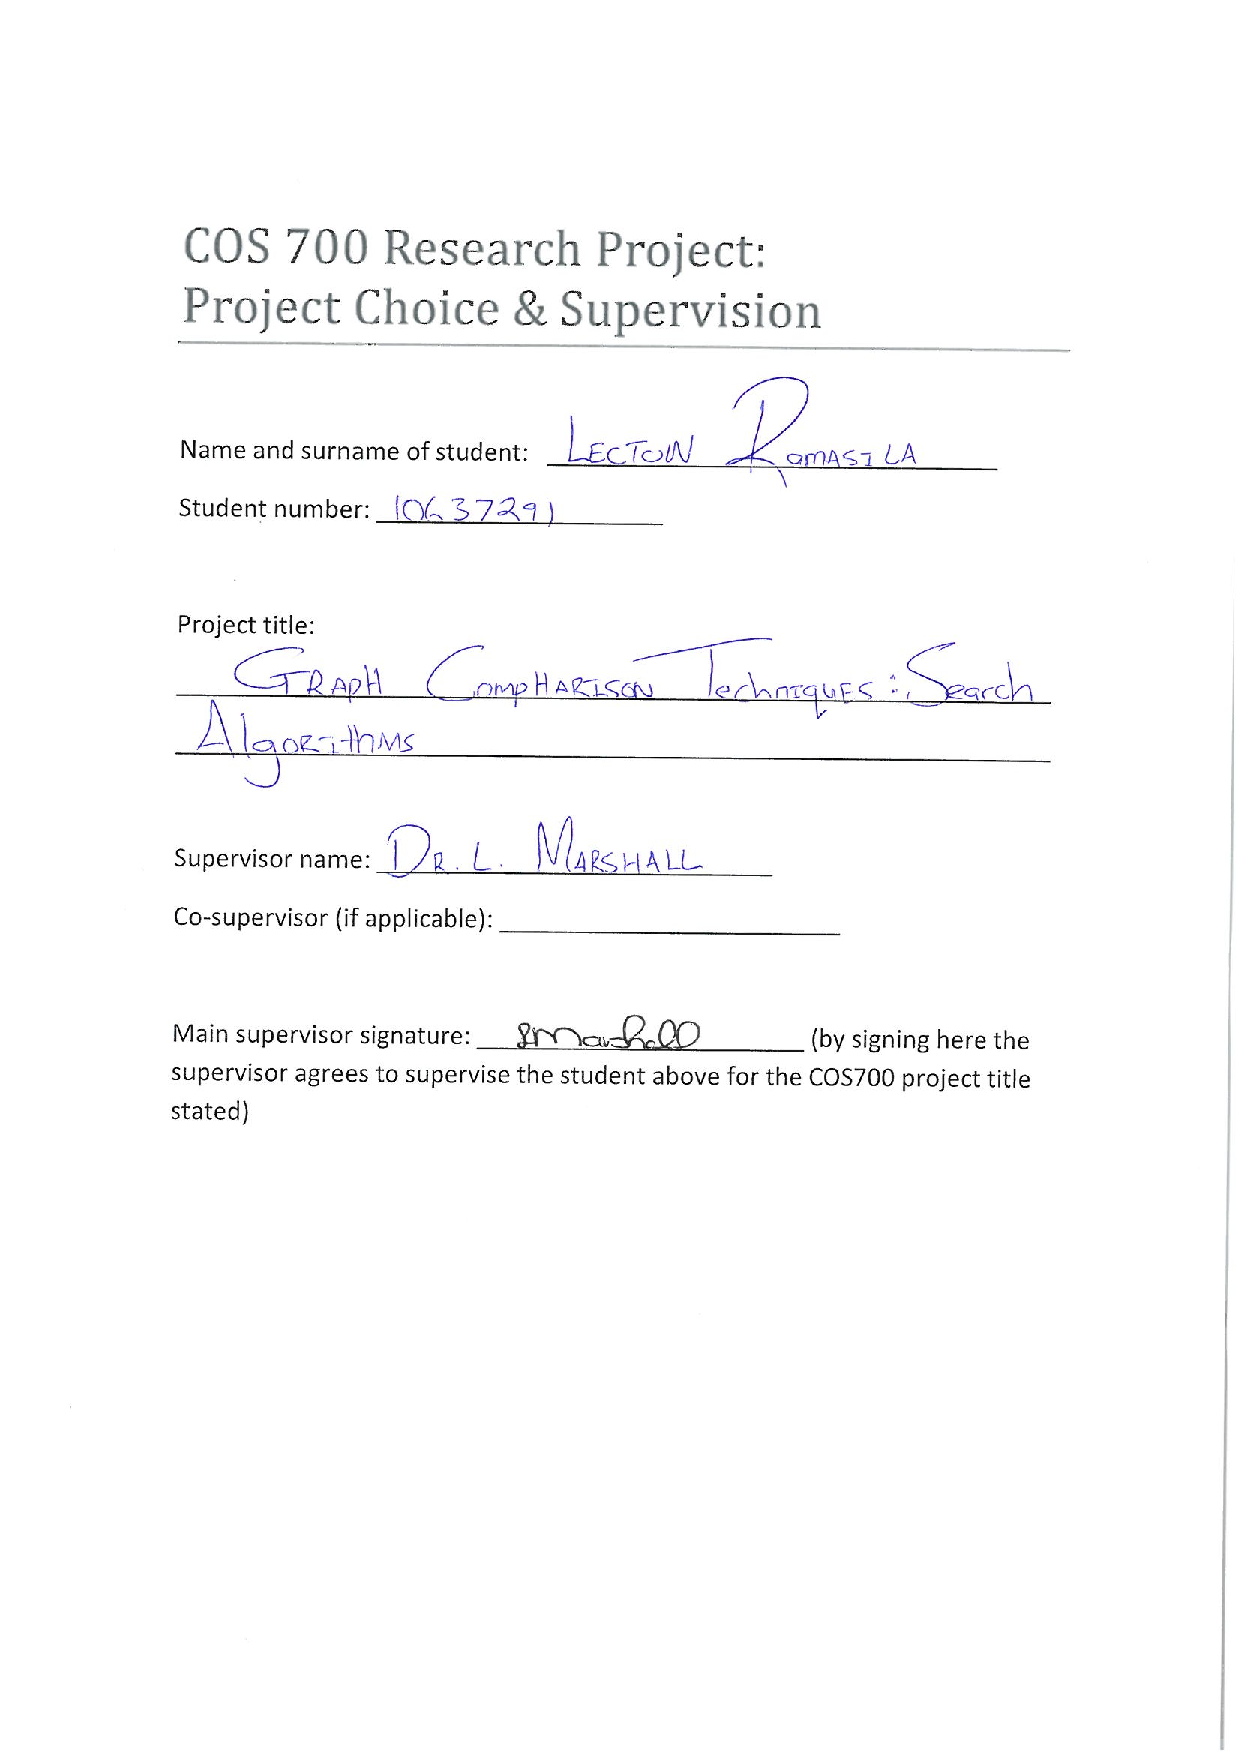
\includepdf[pages={1}]{declaration.pdf}
\begin{abstract}
In this paper, two graph matching algorithms, namely the Ullman and VF2 algrithms, are studied and compared against each other in an attempt to measure their ability to perform syntactic graph comparison efficiently. This
evaluation analysis has practical implications in data warehousing, biochemical applications and E-business. The algorithms take two graphs as input, and they return an association between the two
input graphs. As a result of the comprehensive analysis, we present an argument that considers
the efficiency of the studied algorithms, to determine which amongst them is the best to 
perform graph syntactic comparison.
\end{abstract}
\tableofcontents
\newpage

\subimport{}{Research}

\end{document}  